\documentclass[varwidth=true, border=10pt]{standalone}
\usepackage{tkz-euclide}
\usepackage{tikz}
\usetikzlibrary{patterns}

\begin{document}
\usetkzobj{all}
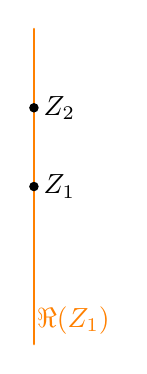
\begin{tikzpicture}
    \tkzSetUpPoint[shape=circle,size=3,color=black,fill=black]
    \tkzSetUpLine[line width=1]
    \tkzInit[xmax=5,ymax=4,xmin=-1,ymin=0]
    \tkzDefPoints{2/2/Z1,2/3/Z2,2/0/A}
    \tkzAxeXY

    \tkzDrawLine[add=2 and 1, color=orange](Z1,Z2)
    \tkzDrawPoints(Z1, Z2)
    \tkzLabelPoint[right](Z1){$Z_1$}
    \tkzLabelPoint[right](Z2){$Z_2$}
    \node[orange] at ($(A)+(0.5,0.3)$)  {$\Re(Z_1)$};
\end{tikzpicture}
\end{document}
